\chapter{Additional Details for Michel Electron Reconstruction}\label{ch:energyfits}

\minitoc

Chapter \ref{ch:michel} provided a study of the fraction energy resolution of
the developed Michel electron reconstruction algorithm, in terms of ionisation
only deposited energy and true Michel electron energy. The gaussian fits used to
estimate the energy resolution and bias as a function of true Michel electron 
energy are given here.

\section{Ionisation Only Energy Resolution}
This section gives the fits used in the estimation of the ionisation only energy
resolution for Michel electrons. The bias and resolution estimates were based on
gaussian fits to the fractional difference between the reconstructed ionisation
energy and the true ionisation energy, which are shown in Figure 
\ref{fig:ionisation_fits}. The data is binned in terms of the total true 
ionisation energy deposited by the Michel electron, and each plot contains the 
data from a single bin. No attempt was made to fit the tails of the 
distribution, which is particularly noteworthy in Figure \ref{fig:ion_fit_25}, 
where there is a significant tail for negative fractional differences. 

\begin{figure}

	\centering
	\begin{subfigure}[b]{0.49\textwidth}
		\centering
		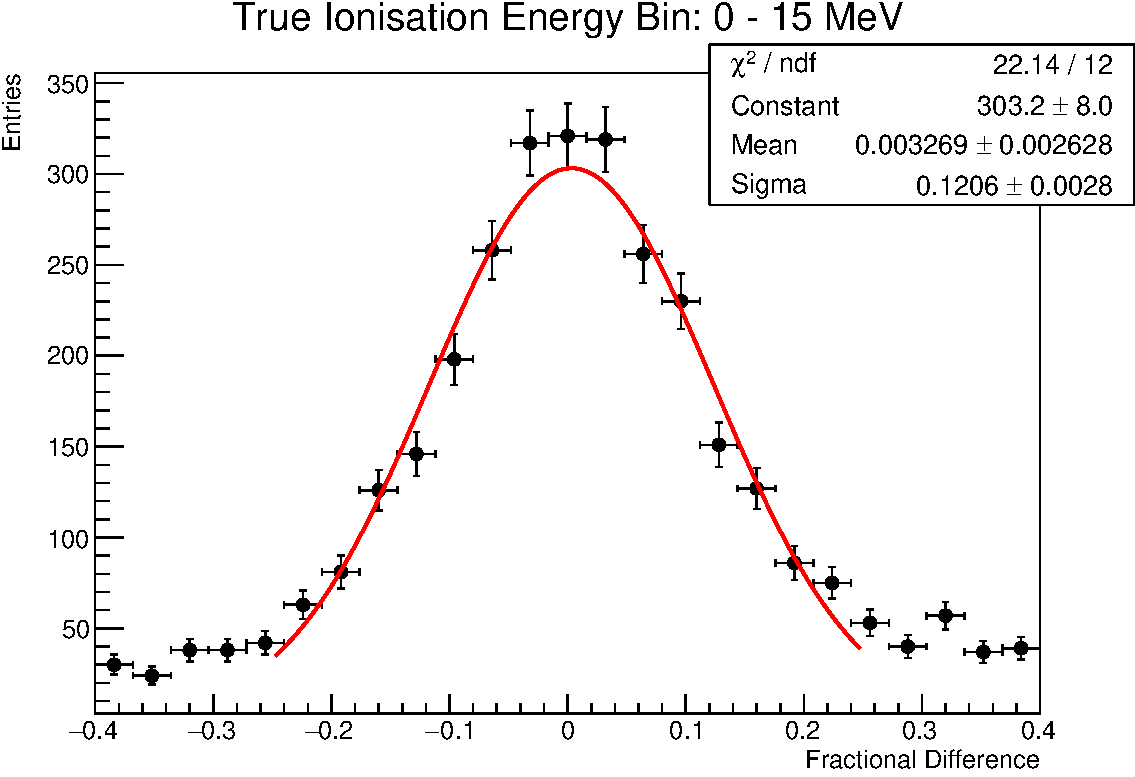
\includegraphics[width=\textwidth]{figures/ion_res_0.pdf}
		\caption {0 - 15 MeV}
	\end{subfigure}
	\hfill
	\begin{subfigure}[b]{0.49\textwidth}
		\centering
		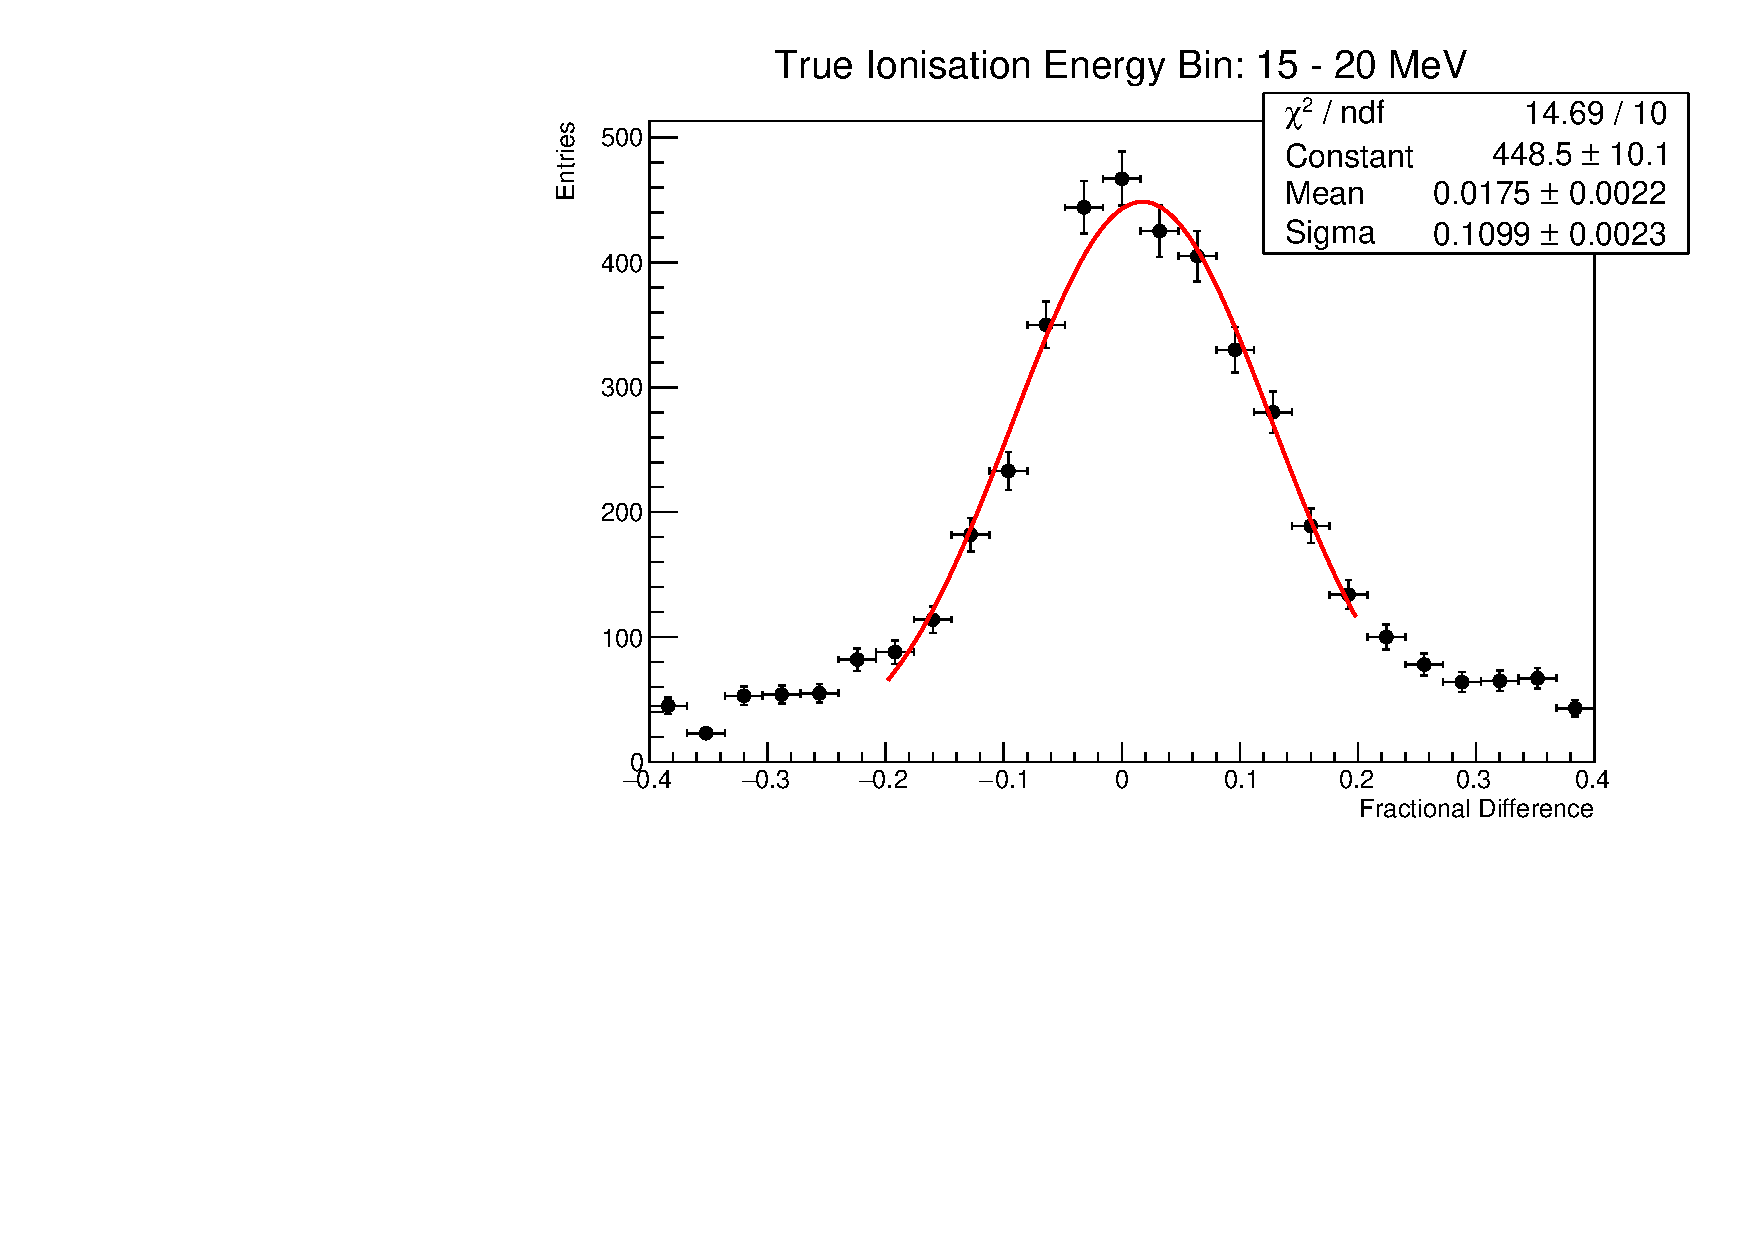
\includegraphics[width=\textwidth]{figures/ion_res_15.pdf}
		\caption {15 - 20 MeV}
	\end{subfigure}
	\begin{subfigure}[b]{0.49\textwidth}
		\centering
		\vspace{5mm}
		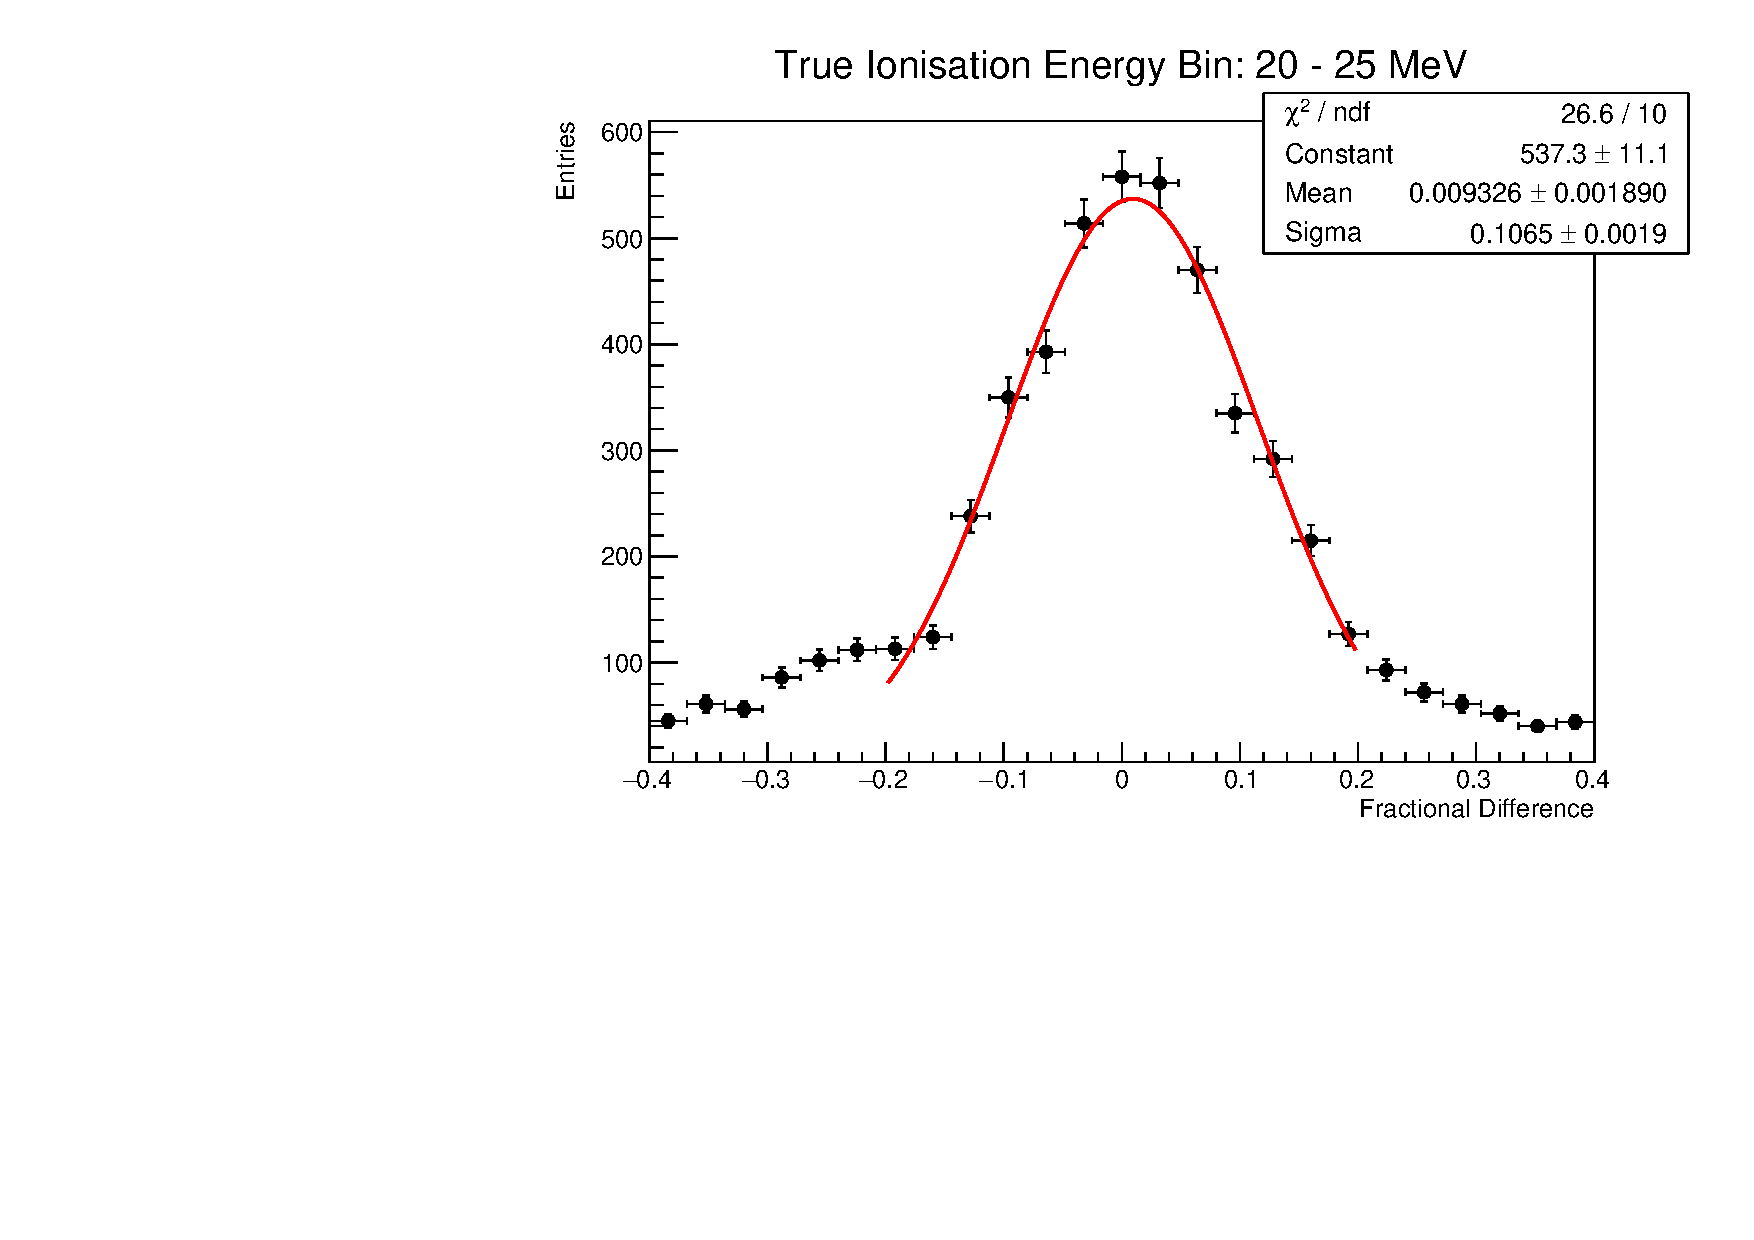
\includegraphics[width=\textwidth]{figures/ion_res_20.pdf}
		\caption {20 - 25 MeV}
	\end{subfigure}
	\hfill
	\begin{subfigure}[b]{0.49\textwidth}
		\centering
		\vspace{5mm}
		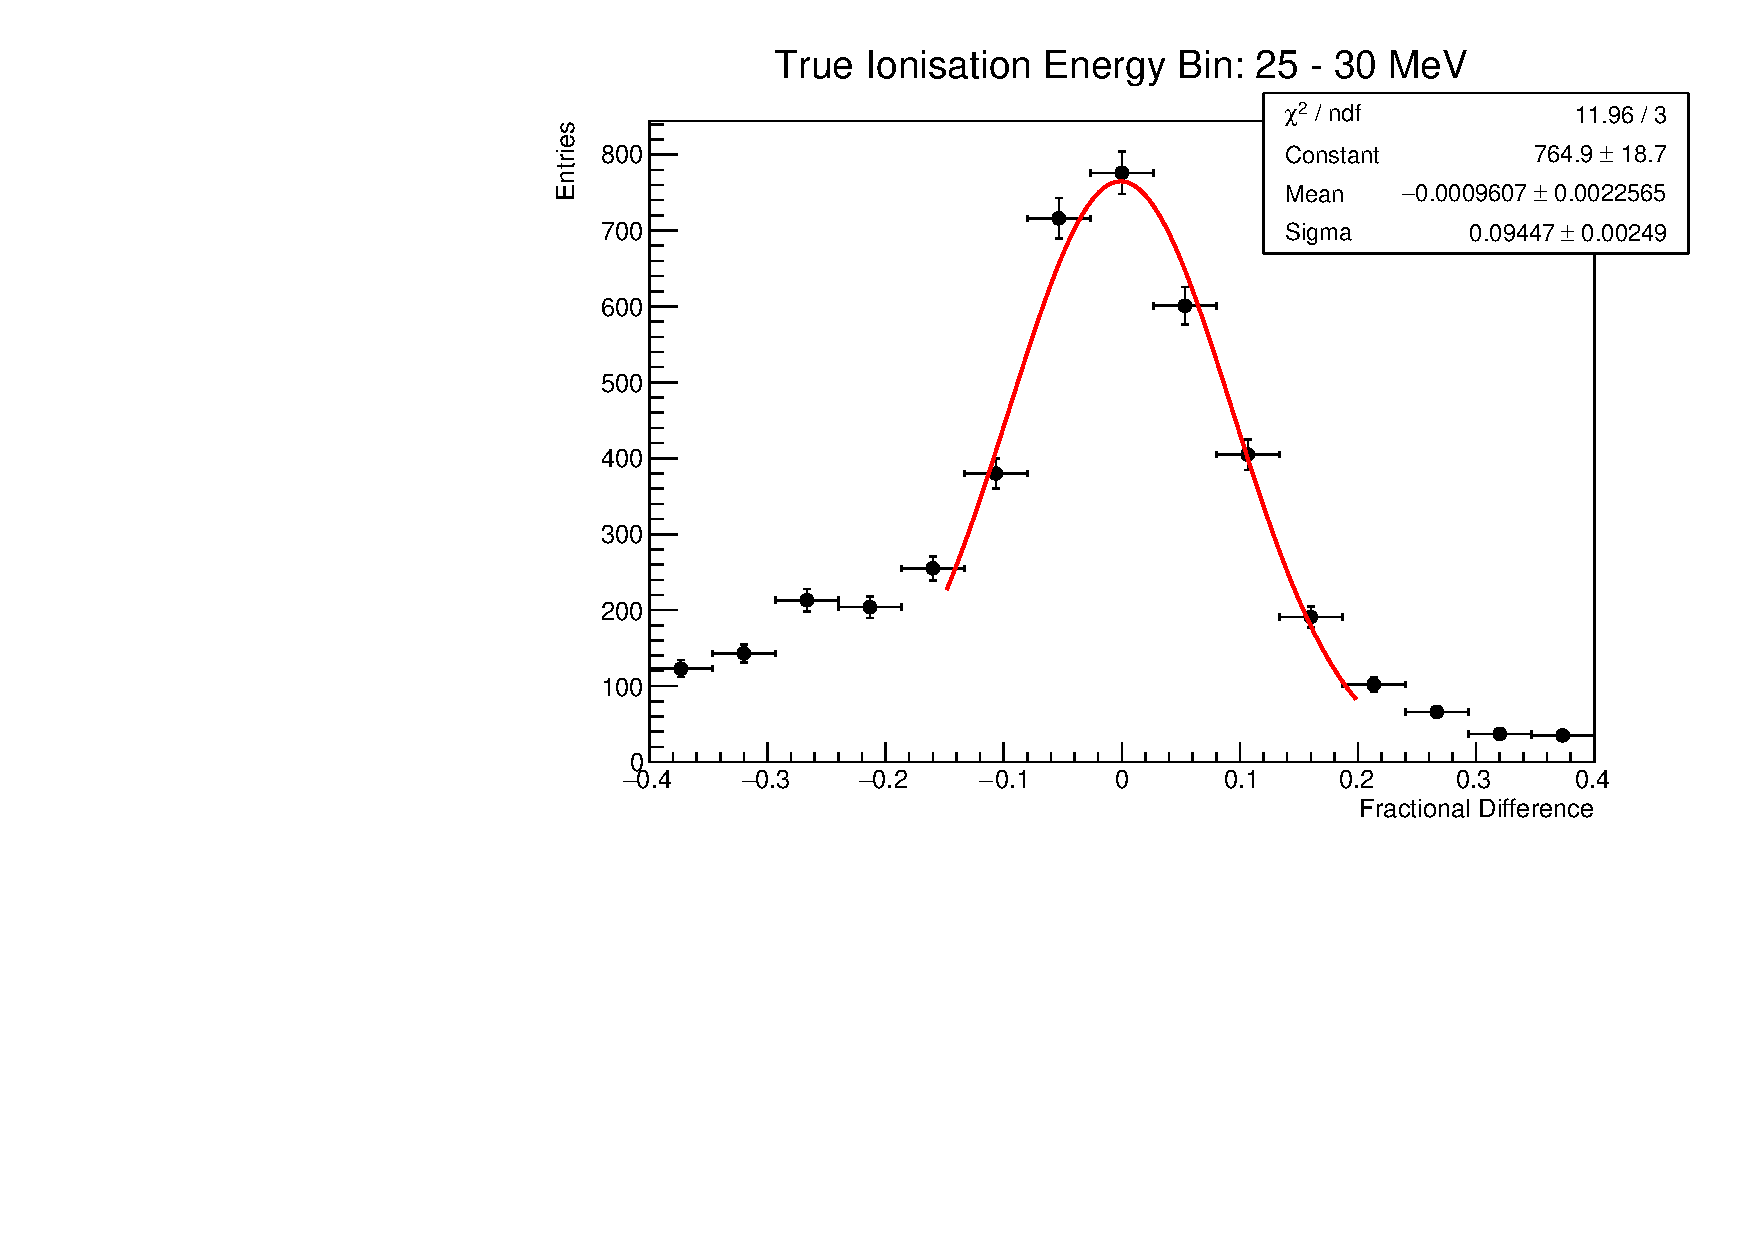
\includegraphics[width=\textwidth]{figures/ion_res_25.pdf}
		\caption {25 - 30 MeV}
		\label{fig:ion_fit_25}
	\end{subfigure}
	\begin{subfigure}[b]{0.49\textwidth}
		\centering
		\vspace{5mm}
		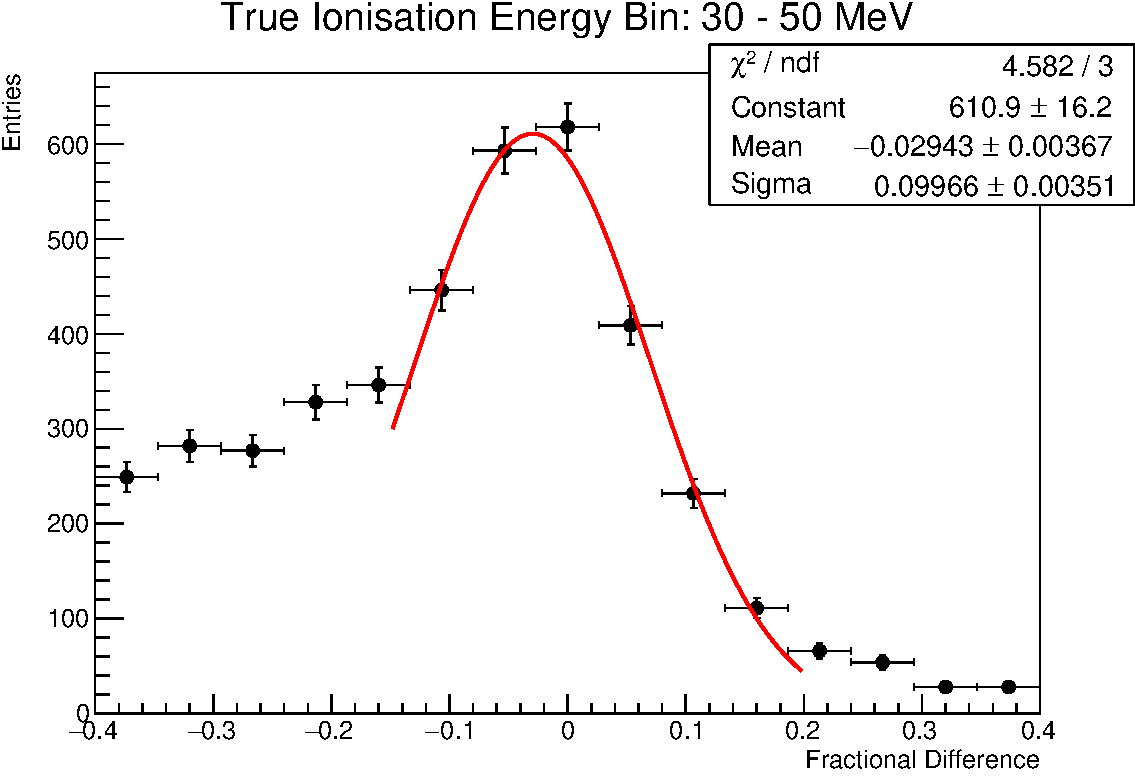
\includegraphics[width=\textwidth]{figures/ion_res_30.pdf}
		\caption {30 - 50 MeV}
	\end{subfigure}

	\caption
	[Gaussian fits to the fractional energy difference bewteen the reconstructed
	ionisation energy and the true ionisation energy for Michel electrons.]
	{Gaussian fits to the fractional energy difference between 
		reconstructed ionisation energy and true ionisation energy, used to predict 
		the energy resolution and bias as a function of energy in Figure 
		\ref{fig:res_and_bias_ion}. No Attempt was made to fit the tails of the
		distribution.}
	\label{fig:ionisation_fits}

\end{figure}

\newpage
\section{Michel Electron Energy Resolution}
\mccorrect{TODO.}
\begin{figure}

	\centering
	\begin{subfigure}[b]{0.49\textwidth}
		\centering
		
\includegraphics[width=\textwidth]{figures/placeholder.png}
		\caption {0 - 15 MeV}
	\end{subfigure}
	\hfill
	\begin{subfigure}[b]{0.49\textwidth}
		\centering
		
\includegraphics[width=\textwidth]{figures/placeholder.png}
		\caption {15 - 20 MeV}
	\end{subfigure}
	\begin{subfigure}[b]{0.49\textwidth}
		\centering
		
\includegraphics[width=\textwidth]{figures/placeholder.png}
		\caption {20 - 25 MeV}
	\end{subfigure}
	\hfill
	\begin{subfigure}[b]{0.49\textwidth}
		\centering
		
\includegraphics[width=\textwidth]{figures/placeholder.png}
		\caption {25 - 35 MeV}
	\end{subfigure}
	\begin{subfigure}[b]{0.49\textwidth}
		\centering
		
\includegraphics[width=\textwidth]{figures/placeholder.png}
		\caption {35 - 50 MeV}
	\end{subfigure}

	\caption{Gaussian fits to the fractional energy difference between
		reconstructed Michel electron energy and true Michel electron energy, used 
		to predict the energy resolution and bias as a function of energy in Figure 
		\ref{fig:res_and_bias_energy}.}
	\label{fig:michel_energy_fits}

\end{figure}
